\chapter{Konzept}
\label{chapter:Konzept}
\myboxy{
	\begin{itemize}
		\item Konzept was speedgoat für die Steuerung und für die Daten Erfassung.
	\end{itemize}
}{To-do}{\textwidth}


Wie in Abbildung \ref{img_1_1:Konzept:0} dargestellt, werden die Baugruppen des Pods an verschiedenen Stellen miteinander verbunden. Dabei übernimmt die Steuereinheit (+SE1) eine zentrale Rolle. Mit der echtzeitfähigen Steuerung von Speedgoat werden alle digitalen und analogen Ein- und Ausgangssignale gesteuert, einschließlich der Distanzmessung und der G-Kraft-Messungen. Die Distanzmessung ist für die Positionsermittlung notwendig, während die G-Kraft-Messung für Forschungszwecke genutzt werden soll. Die Steuereinheit (+SE1) wird von der Batterieeinheit (+BE2) mit Energie versorgt.

\begin{figure}[!ht]
	\begin{center}
		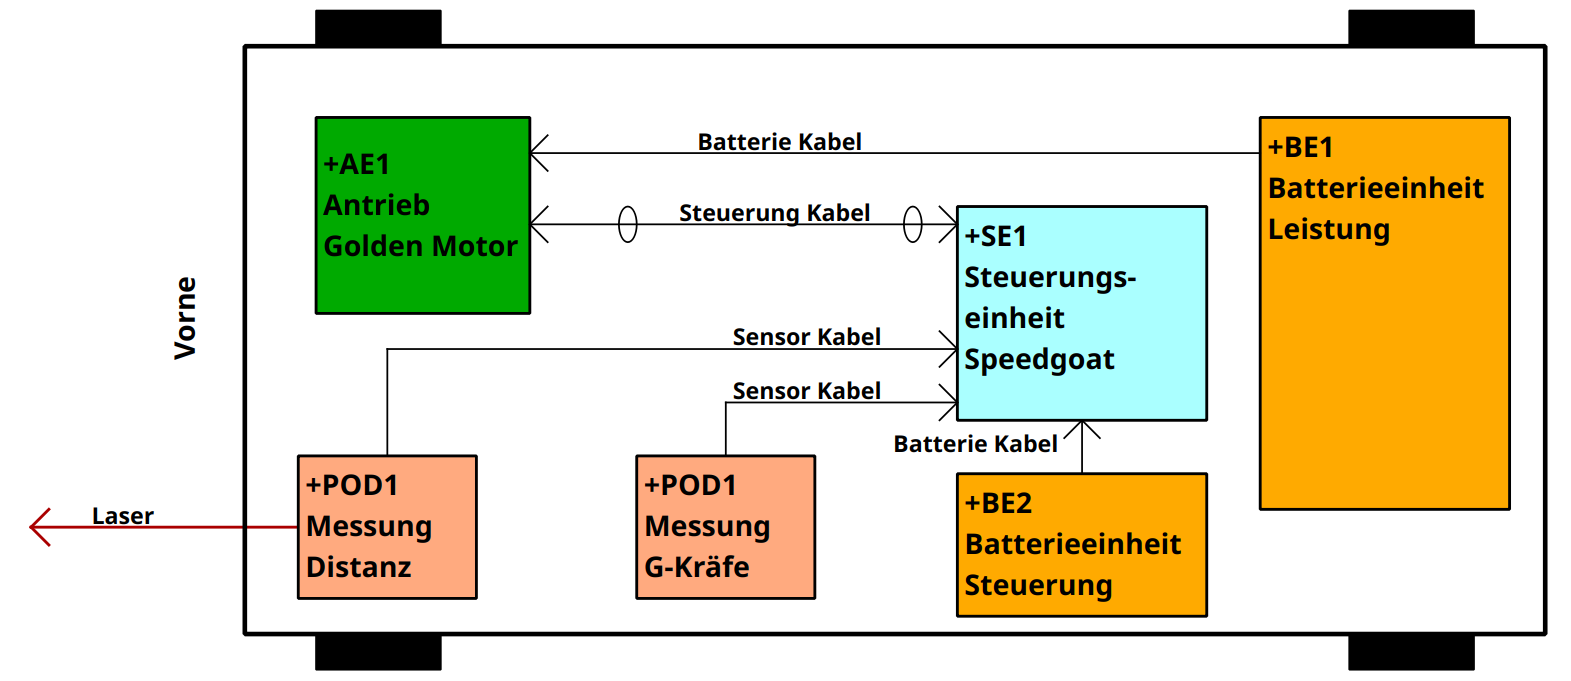
\includegraphics[width=1\textwidth]{img/3_schaltplan/sp_aufbauplan_0.png}
		\caption{Konzept – Aufbauplan des Pods}
		\label{img_1_1:Konzept:0}
	\end{center}
\end{figure}

Der Antrieb (+AE1) erfolgt über einen BLDC-Motor. Dieser wird mittels eines zusätzlichen Steuergeräts, einem Vector-Controller (FOC: Field Oriented Control), angesteuert. Für die Energieversorgung des Antriebs wird eine Leistungsbatterie (+BE1) verwendet.

